%% -*-LaTeX-*-
%%
%% This manuscript has been written using the IEEEtran macros
%% To be submitted to: Open Source Modelling and Simulation of Energy Systems (OSMSES 2022)
%%
%% (c) 2021 Grupo AIA, RTE  
%%
%% 
%%

\documentclass[conference]{IEEEtran}
\usepackage[utf8]{inputenc}
\usepackage{hyperref}
\usepackage{graphicx}
%\usepackage{amsmath,amssymb,amsfonts}
%\usepackage{booktabs}
\usepackage{cite}
\usepackage[cbgreek]{textgreek} % Only for Dynawo "omega" font
\usepackage{xcolor}
\usepackage{listings}
\usepackage{xspace}



%%%%%%%%%%%%%%%%%%%%%%%%%%%%%%%%%%%%%%%%%%%%%%%%%%%%%%%%%%%%%%%%%%%%%%%%%%%%%%%
%% Our short-hand macros
\newcommand{\Dynawo}{Dyna\textomega o\xspace} % unfortunately, it doesn't show in bold
\newcommand{\TODO}{\texttt{TODO:}\xspace}

%% Our colors for backgrounds and code listings
\definecolor{light-gray}{gray}{0.9}
\definecolor{dark-gray}{gray}{0.4}
\definecolor{light-blue}{RGB}{64,64,255}
\definecolor{dark-blue}{RGB}{16,16,64}

%% Our config parameters for code listings
\lstset{
  language=Python,
  backgroundcolor=\color{light-gray},
  basicstyle=\scriptsize\ttfamily,
  keywordstyle=\bfseries,
  identifierstyle=,
  stringstyle=\itshape,
  showstringspaces=false,
  commentstyle=\color{dark-gray}
}

%% Our short-hand macros for code snippets: \console and \code
\lstnewenvironment{console}{\lstset{language=bash}}{}
\newcommand{\code}[1]{\texttt{#1}}

%% More sensible colors for hyperref links
\hypersetup{
  colorlinks = true, % color links instead of ugly boxes
  urlcolor   = blue, % color of external hyperlinks
  linkcolor  = dark-blue, % color of internal links
  citecolor  = red   % color of citations
}





%%%%%%%%%%%%%%%%%%%%%%%%%%%%%%%%%%%%%%%%%%%%%%%%%%%%%%%%%%%%%%%%%%%%%%%%%%%%%%%%
\begin{document}

%% Used by IEEEtran.bst to control some aspects of the bibliography style:
\bstctlcite{BSTcontrol}

% Remember: no symbols, special chars, footnotes, or math in Title or Abstract
\title{Development of an Open Source Tool to Compare Simulators on
  Large-Scale Cases --- Application to Dynawo}
% Previous options for a title:
%%% \title{Black-box validation and A/B testing of large-scale cases
%%%        with DynaFlow and DynaWaltz simulators}

\author{
  \IEEEauthorblockN{
    José Luis Marín\IEEEauthorrefmark{1},
    Vicenç Gaitan\IEEEauthorrefmark{1},
    Guiu Oms\IEEEauthorrefmark{1},
    Adrien Guironnet\IEEEauthorrefmark{2},
    Quentin Cossart\IEEEauthorrefmark{2},
    and Marco Chiaramello\IEEEauthorrefmark{2}}
  \IEEEauthorblockA{
    \IEEEauthorrefmark{1}Aplicaciones en Informática Avanzada SL\\
    Avda. de la Torre Blanca, 57 (Ed.\ EsadeCreapolis)\\
    08172 -- Sant Cugat del Vallès, Spain\\
    Email: \{marinjl, gaitanv, omsg\}@aia.es
  }
  \IEEEauthorblockA{
    \IEEEauthorrefmark{2}RTE R\&D department\\
    7C place du Dôme, 92073 Paris La Défense Cedex\\
    Email: \{adrien.guironnet, marco.chiaramello, quentin.cossart\}@rte-france.com
  }
}

\maketitle

% Remember: no symbols, special chars, footnotes, or math in Title or Abstract
\begin{abstract}
  Dynawo is an open source hybrid Modelica/C++ suite of simulation tools for
  power systems, geared towards the dynamic simulation of large transmission
  networks at different time scales, from the steady-state calculation to
  transient stability analysis. In this paper we present a set of open source
  tools designed for: (a) validation of Dynawo based on black-box testing
  against existing established simulators, or against previous validated
  versions of Dynawo; (b) exploration and analysis of the effects of modelling
  changes and model parameters on the network response, by means of A/B
  testing. In both cases the approach is based on the automatic generation of an
  extensive set of cases derived from a given base case, typically by means of
  N-1 contingencies. Most importantly from the point of view of power systems
  research, a concrete set of metrics is presented here to deal with the
  practical problems of comparing different simulations of large, real-world
  networks. The tools, based on Python and Jupyter notebooks, are designed with
  flexibility in mind, in order to adapt the code to future testing scenarios
  and to extend the metrics used for comparing results.
\end{abstract}

\begin{IEEEkeywords}
  equation based modelling, dynamic simulation, power flow, blackbox validation
\end{IEEEkeywords}




%%%%%%%%%%%%%%%%%%%%%%%%%%%%%%%%%%%%%%%%%%%%%%%%%%%%%%%%%%%%%%%%%%%%%%%%%%%%%%%%
\section{Introduction}

\Dynawo\cite{Guironnet18} is a suite of tools for the dynamic simulation, at
different time resolution levels, of modern power networks.  It has been mainly
developed by RTE, and then released as open
source~\cite{Dynawo}.\footnote{\textcolor{red}{Would you like to briefly mention
  here the relationship to PowSyBl and the Linux Foundation Energy, its use of
  the same IIDM format, etc.?}}  Its design is based on two major guiding
principles: the use of a high-level modelling language
(Modelica~\cite{Modelica}) and a strict separation between the modelling and the
solving mechanisms.  Its implementation brings to the table a novel hybrid
approach that combines the power of declarative, computationally acausal
modelling (also referred to as equation-based modelling) with certain
high-performance C/C++ modifications that take advantage of the specific
optimization opportunities available in large power networks (such as, for
instance, the extensive work on high-performance DAE solvers for these highly
sparse systems).  \Dynawo thus aims at providing power system stakeholders with
a next-generation of open source simulation tools that overcome the limitations
of legacy closed-source programs, while being performant enough to be used in
production settings at large transmission operators. The key goals are
transparency and flexibility of modelling, which will result in robustness and
interoperability. It is hoped that this will enable an effective collaboration
and cooperation in the power system community, something that has been difficult
to achieve with legacy commercial tools.  For a recent update on \Dynawo
developments, see the presentation \cite{Guironnet21} or consult the official
website~\cite{Dynawo}.



\subsection{Objectives of the developed comparison tools}
%\subsection{Aims: not just validation}

%% Stress the possibilites offered by the tool to validate or observe the
%% influence of one parameter or model change on the system reponse, in a
%% systematic way.

Validation of dynamic simulators is hard, and it obviously starts at the level
of individual device models. But, since these devices are increasingly more
complex (with lots of new power electronics and sometimes governed by
algorithmic controls), one needs whole-system functional testing in order to
assess the behavior on complete network cases. As in any hierarchical
system-of-systems, it is not always evident how the lower-level details (device
model choices, parameters, etc.)  affect the behavior of the whole network. This
sort of testing is necessarily ``black-box'' in style, since there is no
systematic way to link the knowledge of the lower-level modelling to the behavior
of the higher-level, other than running simulations---in a certain limited
sense, what we have here is an ``emergent behavior''.  Therefore this sort of
black box simulations are not only useful for validating the software against
previous legacy simulators, or against new versions of the software, but also
for exploring and assessing the effects of different model choices, model
parameters, solver parameters, etc., on the behavior of the whole network,
\emph{in a systematic way}.

The tools presented here aim to fulfill this double role. They leverage modern
rapid development tools from the Python ecosystem (Pandas and Jupyter notebooks,
among several others) to accomplish this. They can automatically create and
configure extensive sets of test cases derived from a given base case, and
efficiently manage large amounts of output. Initially developed for the
validation of \Dynawo at the functional level, they are now also used for the
generation and exploration of extensive sets of cases. These are designed for a
couple of settings: long-term stability studies, with DynaWaltz, and steady
state calculation studies, with DynaFlow.

We also report on the design of an adequate set of \emph{metrics} for comparing
the results from two simulators.  This is a non-trivial problem, which required
experimenting with different choices.  We report on our early experience using
these tools and metrics on recent versions of \Dynawo and using several large
network cases (actual cases from RTE's operational environment, used for
long-term voltage stability studies). Let us now briefly describe the aims and
scope of the tools in each of these two cases.



\subsection{DynaWaltz}

\Dynawo is flexible enough to accommodate several time scales: from
sub-second near-EMT (electro-magnetic transients)~\cite{Masoon21}, to
long-term stability, to steady-state calculation~\cite{Cossart21}
studies. DynaWaltz is the \Dynawo tool used for long-term stability
studies, where the time scales are measured in minutes and the typical
time steps can be of the order of a few seconds. Used in this mode,
\Dynawo simulates the grid in the so-called quasi steady state, and
contains most models impacting the system slow dynamics: tap-changers,
loads, static var compensators, etc.; as well as secondary voltage
regulation and special protection schemes. It is mostly used to study
voltage collapses. Other possible uses in the future may include
cascading failure analysis~\cite{Bialek16}.

Long-term stability studies are a core process of transmission operation whose
role is ensuring power system stability: they consist in analyzing whether the
slow dynamics of the system could lead to an instability or a system
collapse. The validation tools described here were developed to assess and
validate DynaWaltz quantitatively and in a systematic manner, using RTE's
national grid models and cases. DynaWaltz is scheduled to be deployed in
production at RTE (in progressive stages that will start by end of 2021), for
$n$-day ahead operational security studies.

Initially, our overall approach was the use of another
well-established simulator, Astre, which is the currently used tool at
RTE for long-term stability studies, as the reference for comparison
and assessment. More specifically, the validation efforts were focused
on the results obtained for the behavior of the coordinated Secondary
Voltage Control systems. Shortly after, the tools were extended to
accommodate the comparison between different Dyna$\omega$o versions,
or between variations of case models, model parameters, and solver
parameters.



\subsection{DynaFlow}

DynaFlow~\cite{Cossart21} is a novel approach to the calculation of steady states
that leverages the \Dynawo's flexibility for modelling the dynamics at different
time scales. It overcomes an inherent problem that all static power flows have
when presented with controls: discrete event actions, dead-bands, and regulation
limits (control type-switching) all conspire to produce several possible
steady-state solutions, many of them operationally valid.  Static power flows
arrive at a single solution by means of several ``outer loops'' in which
heuristics (accumulated over years of practice) drive the choice of control
changes. However, these heuristics are not bullet-proof (for instance, one may
encounter ``hunting'' oscillations, even with standard tap changers); and more
importantly, they do not take into account the time constants and actual
dynamics of each control. Therefore, even the most principled approaches from the
static power flow camp, such as those based on optimization\cite{Ju20},
complementarity constraints~\cite{Murray15}, or HELM~\cite{Trias18} cannot
guarantee arriving at the correct solution, since they are blind to the the
different dynamics of different competing controls.

In the current scenario, where more complex power electronic devices
and complex algorithm-based controls are being introduced each year,
this problem is getting worse. DynaFlow solves these types of problems
by simulating the network in the time domain and using the actual time
constants that govern the actions of relevant controls. It also
contemplates protection schemes, including modern Special Protection
Schemes (SPS), thus opening the door to the realistic simulation of
cascading effects in contingency studies and interactions between
controllers.

Following the work done for DynaWaltz validation, we built a similar
set of tools for the validation of DynaFlow, as well as the
exploration of extensive sets of (contingency) cases.  Again, the
approach to validation is based on comparison against a
well-established power flow, Hades 2, which is the currently used tool
at RTE for steady state calculation. But in addition, the tool is also
prepared for comparing different DynaFlow versions, and more
generally for assessing the effects of varying the case models, model
parameters, and solver parameters.


%%%%%%%%%%%%%%%%%%%%%%%%%%%%%%%%%%%%%%%%%%%%%%%%%%%%%%%%%%%%%%%%%%%%%%%%%%%%%%%%
\section{Structure and workflow}
%% \begin{center}
%%   \itshape
%%   Outline:
%%   \begin{itemize}
%%     \item High-level structure of the tools: preparatory steps, pipeline,
%%           analysis/exploration of outputs.
%%     \item Preparatory steps: the BASECASE. Requirements and other conventions
%%           assumed.
%%     \item Pipeline: general structure and steps involved. Design
%%           decisions. Parallelization. Storage Considerations.
%%     \item Analyzing the results: Jupyter notebook; output of metrics to
%%           file for further analysis with other tools.
%%     \item Other stuff: auditability of results (logs); reconstructing
%%           cases from the basecase and reproducing runs. Example: grepping for
%%           common modes of failure in log files --> uncover systematic problems
%%           appearing in a specific model, for instance.
%%     \item Typical workflows (for instance, start small with a small random
%%           sample of contingencies; then ramp up to full N-1 list. Or settle on
%%           a custom list of ``most interesting'' contingencies via regexes.)
%%     \item \textbf{Fig} of the block architecture for all this.
%%   \end{itemize}
%% \end{center}

Here follows a high-level description of the structure of the tools,
along with the typical workflow that the user is expected to carry out
when using them.  For the details on installation instructions and its
requirements, please refer to the software documentation on the GitHub
repository, which is to be located under the main Dyna$\omega$o
project pages~\cite{DwoGitRepos}.

As described above, this validation system is based on comparing
results against a well-known reference system. In our case, this was
the Astre simulator for the validation of DynaWaltz, and Hades 2 for
the validation of DynaFlow. The cases used for comparison are
essentially all possible single-element disconnections (shunts, lines,
etc.). Therefore the tools are currently oriented towards the
generation of contingency cases derived from a given base
case. However, the design is quite modular; it is easy to modify the
corresponding scripts so that the set of cases would be something
other than contingencies, such as, for instance, variations of a given
set of model parameters, or the solver time-step, etc.

Viewed at a the highest level of abstraction, the tools are structured
to follow this basic workflow:
\begin{itemize}
\item Prepare the ``base case'' (this is aided by some helper scripts,
  but it's a semi-manual task)
\item Create a number of study cases derived from the base case, run
  them, and collect all results into suitable common formats for
  comparison analyses (this is fully automated)
\item Analyze the results (pre-configured and ready-to-use Jupyter
  notebooks)
\end{itemize}
In order to describe the tool components, let us now see this workflow
in detail. From a functional point of view, the steps are:
\begin{enumerate}
  \item Obtain a study case containing the two set of files that
    (purportedly) represent the same case, i.e.~the DynaWaltz and
    Astre (or DynaFlow and Hades 2) files;
  \item Prepare the base case: standardize the folder and file
    structure (see below), the XML formatting, and possibly some
    case-specific input (such as which curves to extract, for
    instance);
  \item Create the contingency cases derived from the base case: for
    each type of device whose disconnection is supported (shunts,
    loads, generators, lines, transformers), create the specified
    number of single-contingency cases.
  \item Run Astre/Hades 2 and DynaWaltz/DynaFlow on the contingency
    cases, collecting results and logs into organized (and compressed)
    storage;
  \item Extract result data in a format common to Astre/Hades 2 and
    DynaWaltz/DynaFlow;
  \item Compute \emph{metrics} on the results obtained (this may
    include variables of the final steady state, or curves and
    selected automata event history, or both);
  \item Use the Jupyter notebook to browse and analyze the results,
    and obtain lists of contingency cases that can be ranked according
    to various compound scores built on those metrics;
  \item Further analysis is possible using these ranked tables that
    the notebook exports to CSV files (e.g. using Excel).
\end{enumerate}

Steps 1 and 2 are concerned about preparing the main input to this
whole process, i.e.~the base case, in a suitable format for its
automated process. This should contain two cases for performing an A/B
comparison analysis. The tools are prepared to compare \Dynawo
vs.\ \Dynawo as well as Astre vs.\ \Dynawo and Hades 2
vs.\ \Dynawo. Obviously one should firstly make sure that the A \& B
files do correspond to the same case. This is relatively easy when
both cases are \Dynawo, but challenging when the simulators are
different.  One needs not only the underlying network model to be the
same, but additionally the identifiers of at least the most basic
elements (buses, loads, generators, etc.) to be the same, or provide a
way to find a one-to-one correspondence in order to match them.  In
our experience at RTE, even having a single-source asset database
feeding the creation of both files was not enough to have 100\%
matching of all elements---there would always be a small number of
non-matching devices, such as, for instance, in the case of merged
loads, or different bus-branch vs. node-breaker
representations. Therefore the tools take this into account, only
disconnecting elements and comparing variables that can unequivocally
be matched between the two.

Beginning with Step 3, the rest of this workflow has been automated
through a series of Python programs and Bash shell scripts. Tied
together, we will refer to this system as the \emph{process pipeline}
for validation. This is depicted schematically in
Figure~\ref{fig:pipeline1}. Each script in this pipeline can also be
run individually, either for debugging purposes or just because one
wants to run the pipeline manually step by step.

\begin{figure}
  \centering
  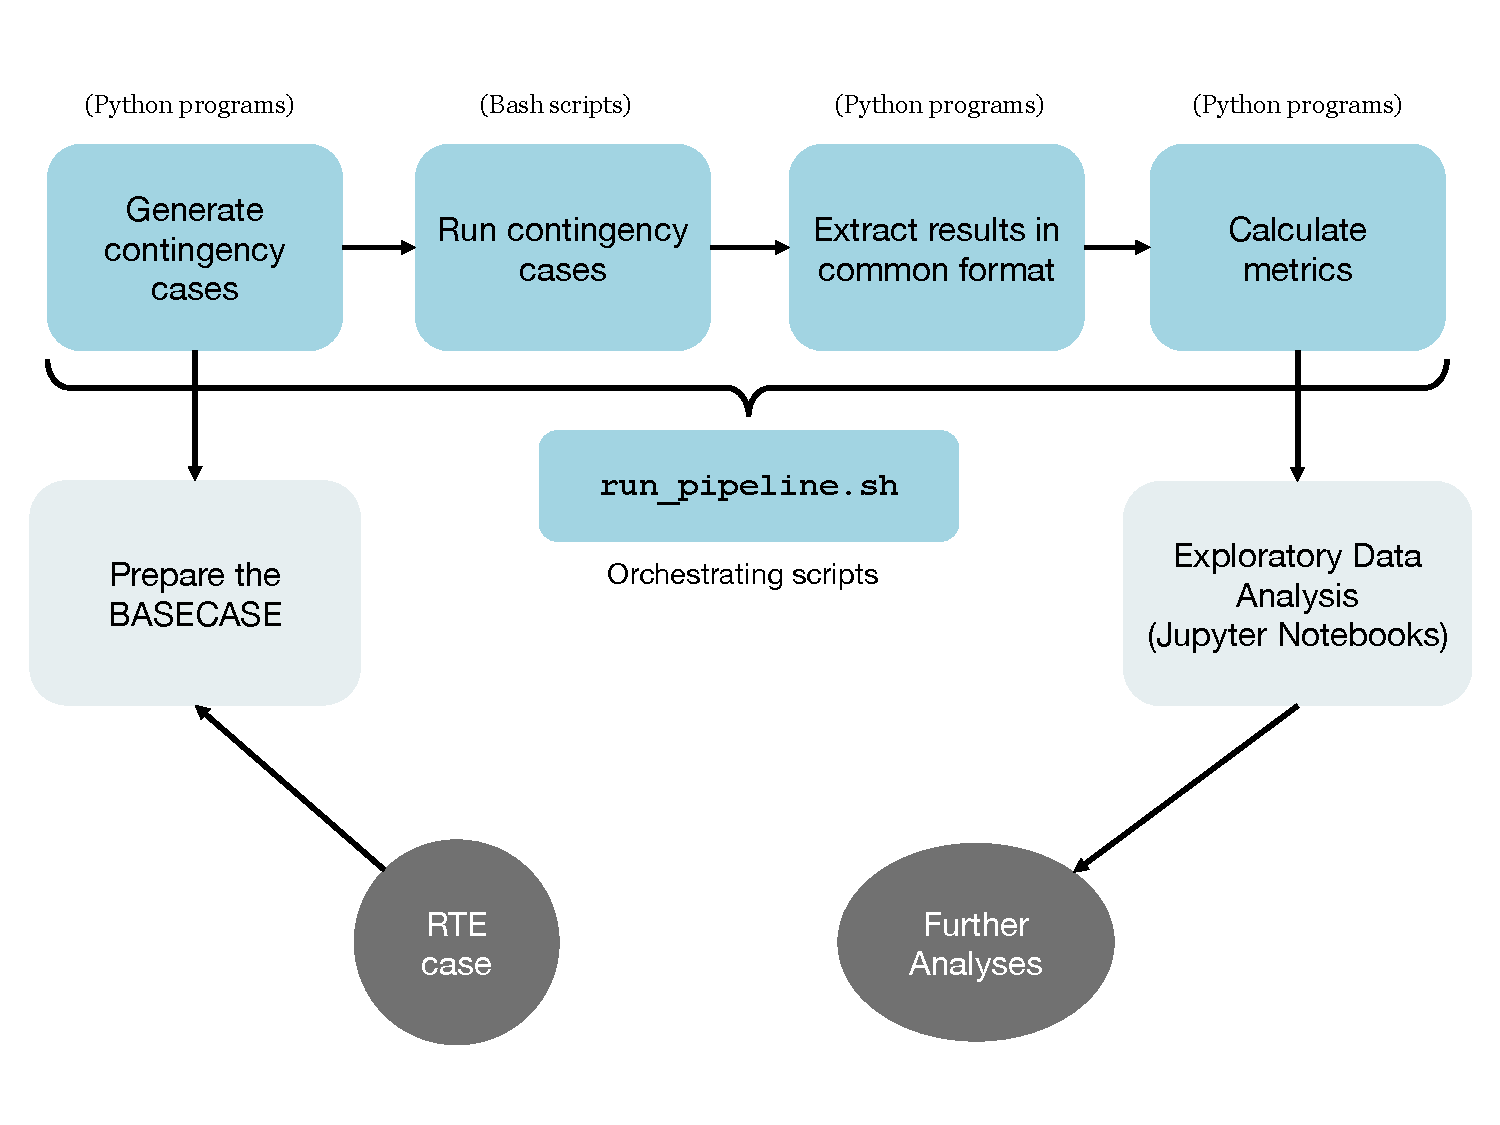
\includegraphics[width=0.48\textwidth]{figs/pipeline}
  \caption{The processing pipeline for validating DynaWaltz against
    Astre, based on contingency cases. The pipeline for DynaFlow
    vs.~Hades 2 follows the same architecture. In both cases, one can
    also compare Dynawo vs.~Dynawo cases (or different versions of
    Dynawo).}
  \label{fig:pipeline1}
\end{figure}

The modularity of this design and the use of scripting languages
allows for rapid changes and adaptation to other testing
scenarios. For instance, our implementation creates comparison cases
based on single-element contingencies derived from a common base case,
but other users may want to use a different criterion. This can be
achieved by replacing only the script that generates the set of
comparison cases, while the rest of the pipeline would remain the
same.

In the following we describe the components of this pipeline, separately
for DynaWaltz and DynaFlow.


\subsection{Details for DynaWaltz}

In terms of preparing the input (Steps 1 and 2 above), the system requires a
valid case in which the DynaFlow and Astre files (or the two DynaWaltz files, in
case of \Dynawo vs.\ \Dynawo comparison) should correspond to the same grid
model, same simulation time, and same disconnection events.  They should be
arranged with a specific folder and filename structure, although there are very
few hard-coded assumptions:
\begin{itemize}
\item All the files comprising the case should be stored under one
  single directory (the name of this parent directory is free).
\item In the case of \Dynawo vs.\ Astre comparisons, the Astre case
  should be in a sub-folder named ``Astre'', and the DynaWaltz case
  should sit at the first level of the directory. Actually, only the
  \Dynawo ``job'' file is required to be there--the rest of \Dynawo's
  input files are inferred from the job file and could sit inside
  sub-folders, as they typically are.  However, the job file name
  should contain the word \code{JOB} and have XML extension in order
  to be identified.
\item In the case of \Dynawo vs.\ \Dynawo, the job files should sit at
  the first level of the directory, their names should contain the
  word \code{JOB\_A}, \code{JOB\_B}, and have XML extension. The rest
  of \Dynawo's input files are inferred from the job file, but it is
  recommended that they are separated into sub-folders \code{A} and
  \code{B}. A utility script is provided in order to restructure base
  cases using these conventions.
\end{itemize}
Both cases should define at least one disconnection event, whose time will be
used as the reference for all generated contingency cases.  Additionally, they
should provide a set of ``curves'', i.e. a selected set of variables to be
output (value vs.\ time) by the simulation. A helper script
(\code{prepare\_basecase\_curves.py}) is provided to prepare these curves so that
the variable names coincide between DynaWaltz and Astre. All generated
contingency cases will then contain this common set of curves--plus a few more
related to the specific contingency.

On the other hand, there are a few optional arrangements that can result in very
significant storage and CPU time savings, particularly when tens of thousands
of contingencies are created and run.  Some are trivial, such as reducing the
log level, eliminating unnecessary output files from the job file, or
re-indenting all XML files in order to produce smaller diffs (contingencies are
stored as incremental diffs over the base case). But some are more subtle: for
DynaWaltz, simulations are normally structured in two stages (labelled \code{t0}
and \code{tFin} at RTE); this is done so that one may apply a change in the
first stage (such as a load increase, for instance) and let things stabilize to
a new steady state, prior to applying a disconnection (or any event of interest)
in the second stage.  In this case, one should prepare the base case so that the
\code{t0} stage has been run, and then edit the job file to remove it while also
editing the \code{tFin} stage to point to a common shared location for the
\code{t0} result files. Done this way, one will not needlessly run the
simulation of the t0 stage in each of the contingency cases, as it is identical
to all of them.

The rest of the steps are fully automated as a pipeline of shell scripts and
Python modules, as depicted in Fig.~\ref{fig:pipeline1}:
\begin{itemize}
\item \code{create\_*\_contg.py}: generate single-element contingency cases
  (generators, loads, shunts, lines, transformers), either as a specified list
  (allowing regular expressions), a random sample, or the exhaustive list.  Most
  of the difficulties in constructing this system lie in this module, as one
  needs to be sure that the disconnection event and the extracted output
  variables do represent the same magnitudes and refer to the same
  devices. Contingency cases are created only when such match can be found (in
  our case, this was done via the asset IDs); this means that sometimes there
  are fewer cases than expected, as it happens for instance when there are
  differences in the way that equivalent loads are merged, or in bus-branch
  vs.\ node-breaker representation choices.
\item \code{run\_all\_contg.sh}: run \Dynawo and Astre on all generated
  contingency cases, with the option of spawning jobs in parallel if several
  CPU cores are available (it uses GNU parallel).  A lower-level script
  (\code{run\_one\_contg.sh} takes care of collecting and compressing all
  results and log files, erasing the contingency cases. It also calls a module
  (\code{extract\_automata\_changes.py}) to extract data about about certain
  events; in our case, transformer taps, shunt bank changes, and secondary
  voltage control actuation.
\item \code{calc\_*\_diffmetrics.py}: compute various metrics for
  comparing results from both simulators. This is done separately for
  curve data and for automata events. Section~\ref{sec:metrics} below
  describes these.
\item \code{top\_10\_diffs.py}: compute a summary report with the most salient
  differences found across various variables of interest and across the whole
  set of contingencies, in order to quickly assess global results ``by-eye''.
\item \code{generate\_notebooks.py}: convenience script that copies the main
  Jupyter notebook to the results directory and configures it with the required
  paths to the data files. This notebook is the main tool for exploratory work
  and deeper analysis.
\end{itemize}
Orchestrating this whole process, we have a high-level driver script,
\code{dynawaltz\_run\_pipeline.sh}. This would be the launcher to call when
scheduling a non-interactive batch job with cron, for instance.



\subsection{Details for DynaFlow}

The system for DynaFlow was constructed later and therefore benefited from the
experience gained with the experimentation and trials done for the validation of
DynaWaltz. It is organized along the same philosophy and structure, so for
brevity, only a few significant differences will be highlighted. 

As before, the process entails a few semi-manual steps for preparing the base
case (aided by some utility scripts), and then a fully automated pipeline that
creates contingency files, runs the simulations, extracts and stores the output
data efficiently, computes several metrics of interest, and finally produces a
summary of differences and a Jupyter notebook for deep analysis of the results.
What is different is that in this case the solution of interest is the final
steady state power flow, and therefore all data and metrics involved are
completely different. Since Hades is a static power flow engine, the time-domain
evolution of continuous variables and discrete events (protection relays, taps,
shunts, etc.) cannot be compared; but if curves are configured for DynaWaltz,
their output is kept, as they are useful for understanding the root cause of
large differences.  This is, after all, one of the main \emph{raisons d'être}
for DynaFlow, namely its ability to calculate a more correct steady state thanks
to a dynamic simulation that takes into account the different time constants of
overlapping and possibly competing controls (let alone protection relays).

These are the components of the pipeline, whose naming and structure mirrors the
DynaWaltz pipeline shown above:
\begin{itemize}
\item \code{create\_*\_contg.py}: generate single-element contingency cases.
\item \code{run\_all\_contg.sh}: run \Dynawo and Hades on all generated
  contingency cases, in parallel if several CPU cores are available.  It calls
  (\code{run\_one\_contg.sh} (to collect and compresses results and logs) and
  \code{extract\_powerflow\_values.py} (to extract the power flow in a common
  format), and \code{extract\_automata\_changes.py} (to extract tap, shunt, and
  secondary voltage control events).
\item \code{calc\_global\_pf\_diffmetrics.py}: compute various metrics
  for comparing the power flow results from both
  simulators. Section~\ref{sec:metrics} below describes these.
\item \code{top\_10\_diffs.py}: compute a summary report of the most salient
  differences found.
\item \code{generate\_notebooks.py}: convenience script that copies and
  configures the main Jupyter notebook to the results directory.
\end{itemize}
Orchestrating this whole process, we have a high-level driver script,
\code{dynaflow\_run\_pipeline.sh}.





%%%%%%%%%%%%%%%%%%%%%%%%%%%%%%%%%%%%%%%%%%%%%%%%%%%%%%%%%%%%%%%%%%%%%%%%%%%%%%%%
\section{Metrics, visualization, and validation}
\label{sec:metrics}

The quantitative comparison of results coming out of different dynamic
simulators is often a challenge, but it becomes highly nontrivial
when dealing with large scale, real transmission networks. It is
assumed here that one is past the stage of having validated the
simulators at the level of very simple networks with one or two buses,
where device models can be unitarily tested, isolated from complex
collective interactions. Here, instead, one wants to test and measure,
as quantitatively as possible, the behavior of the simulators in the
real world---verification and validation of the integrated system.
The difficulties lie on several issues: (a) The sheer number of
variables, which requires one to properly \emph{reduce the data} in
order to attempt any comparison; (b) The fact that the network
dynamics is often \emph{sensitive} to small changes, so that slight
differences produced at one point may quickly amplify down the time
line. This is clearly the case in thresholding effects, i.e. when a
magnitude is close to triggering some actuator (protection relays,
shunts, taps), which is a sure recipe for obtaining different results
from two simulators.

Still, the work reported here has shown us that it is feasible to
devise data reduction techniques and metrics to obtain quantitative
results, which combined with rapid exploration and analysis of
the results (greatly aided by good visualization choices) allows one to
validate simulators via an extensive set of test cases (in our case,
exhaustive $N$-1 contingency runs).

Conceptually, we adopted the following itinerary:
\begin{enumerate}
  \item Begin by selecting the \emph{``signals''} to be
    used for the comparison. Which output variables and events should
    be considered, and which should be discarded? --- Because it's simply
    not manageable nor practical to compare all of them.
  \item Then generate a suitable \emph{reduced set of parameters} that
    characterize each type of signal. ---  Because one is not interested
    in perfect waveform accuracy (in the case of curves), or in
    perfect event timings (in the case of automata events).
  \item Then design the \emph{metrics} for measuring the distance
    between the two simulator results in the space of said reduced
    parameters.
  \item Design effective visualizations. This is essential not only
    for the final tool, but as a critical aid in guiding the design of
    metrics.
  \item Define validation \emph{thresholds} for each class of such
    metrics, which are necessary for establishing hard pass/fail
    criteria (useful when automating tests).
  \item Define one or more \emph{compound scoring} schemes for ranking
    cases. The reduced parameters belong to very disparate classes
    (say, for instance, change in steady-state bus voltages
    vs.\ changes in Mvar peak-to-peak amplitudes); therefore we need
    to decide how to combine these into a single figure of merit, for
    the purposes of ranking and sifting the worst cases that need our
    attention.
\end{enumerate}
Of course, this process was not linear; it entailed feedback loops and
repeat cycles until the research converged on the most adequate or
most effective design decisions, guided by the obtained results.  Each
of these conceptual steps is now discussed in detail.



\subsection{DynaWaltz metrics}

\subsubsection{Selection of signals}
Here we use the word \emph{signals} to refer to both time-dependent continuous
variables such as voltages and (P,Q) values, as well as discrete events such as
actions fired by control automata.  Many times we refer to signals of the
first kind as \emph{``curves''}, since this is the terminology used for the
output in both Astre and Dynawo. For signals of the second kind, we will
call them \emph{``automata events''}, or simply automata.

Since DynaWaltz is specifically targeted towards long-term voltage
stability studies, our validation criteria have been focused on the
behaviour of the coordinated Secondary Voltage Control (SVC)
systems. This means that, among the huge number of possible signals
available from the simulation, the comparison looks only at these:
\begin{itemize}
\item 4 types of variables related to the SVC systems: pilot bus
  voltages, control K-levels (the gain), and (P,Q) of participating
  generators.
\item the bus voltage(s) of bus(es) involved in the particular
  contingency for each case.
\end{itemize}
Additionally, the criteria also contemplate certain automata events:
\begin{itemize}
  \item Transformer taps (up / down) --- anywhere
  \item Load-transformer taps (up / down)
  \item Shunt capacitor \& reactor banks  (connections / disconnections)
\end{itemize}
In the case of automata events, they are contemplated across the whole
network. The base test cases we used correspond to the whole of
France, down to the 45kV level.

Note that K-levels of SVC systems are discrete in nature and each
change in their value also appears logged in the output as events, but
it is much easier to deal with them as curve data.


\subsubsection{Reduced set of parameters}
Here the aim is to distill a reduced set of parameters that
characterize the whole signal sufficiently well for our purposes. It
is then on these reduced magnitudes that we will define the metrics.
Since these are transient signals and we are not really interested in
matching the detailed waveforms with high fidelity, we will try to
focus on electrically relevant features.  After contemplating and
testing a few options, we came up with the following set of 5 reduced
parameters for curves:
\begin{description}
\item[dSS:] \hfill \\ ``delta-SS'', i.e. the difference in signal value between
  the initial steady state and the final steady state.
\item[dPP:] \hfill \\ ``delta-PP'', i.e. the peak-to-peak amplitude of the
  signal during the transient.
\item[TT:] \hfill \\ transient time, i.e. the duration of the transient.
\item[period:] \hfill \\ period of the main component of the transient, as
  obtained by Prony analysis.
\item[damping:] \hfill \\ damping of the main component of the transient, as
  obtained by Prony analysis.
\end{description}

For automata events, and more precisely for tap and shunt events, we have
devised a reduced set of 3 parameters that mimic dSS, dPP, and TT, respectively:
\begin{description}
\item[netchange:] \hfill \\ net change in tap value (or in connection status,
  for shunts) between the initial steady state and the final steady state.
\item[p2pchange:] \hfill \\ peak-to-peak change in tap value during the
  transient.
\item[numchange:] \hfill \\ total number of tap changes (or connection /
  disconnections, for shunts) in the transient.
\end{description}

Figures~\ref{fig:tcharacteristics1} and ~\ref{fig:tcharacteristics2} below show
all these parameters graphically.

\begin{figure}
  \centering
  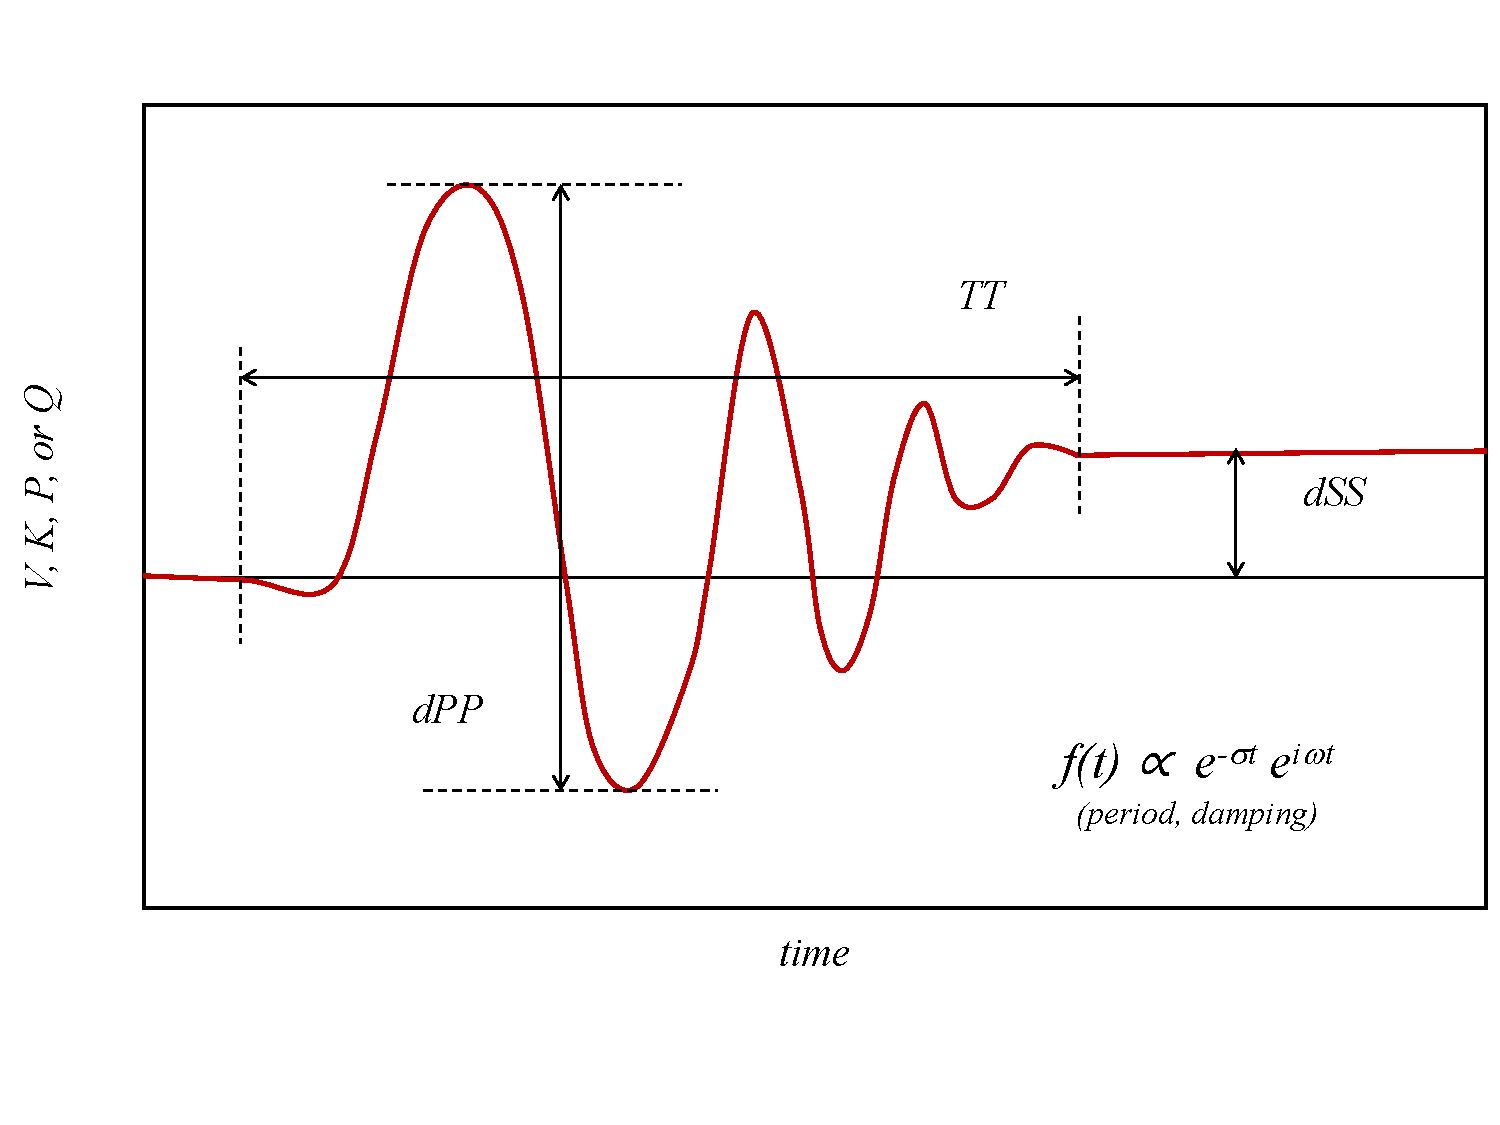
\includegraphics[width=\columnwidth]{figs/transient_characteristics_1}
  \caption{Our selection of reduced parameters for characterizing a
    continuous time-dependent transient signal, for the purposes of
    estimating differences.}
  \label{fig:tcharacteristics1}
\end{figure}

\begin{figure}
  \centering
  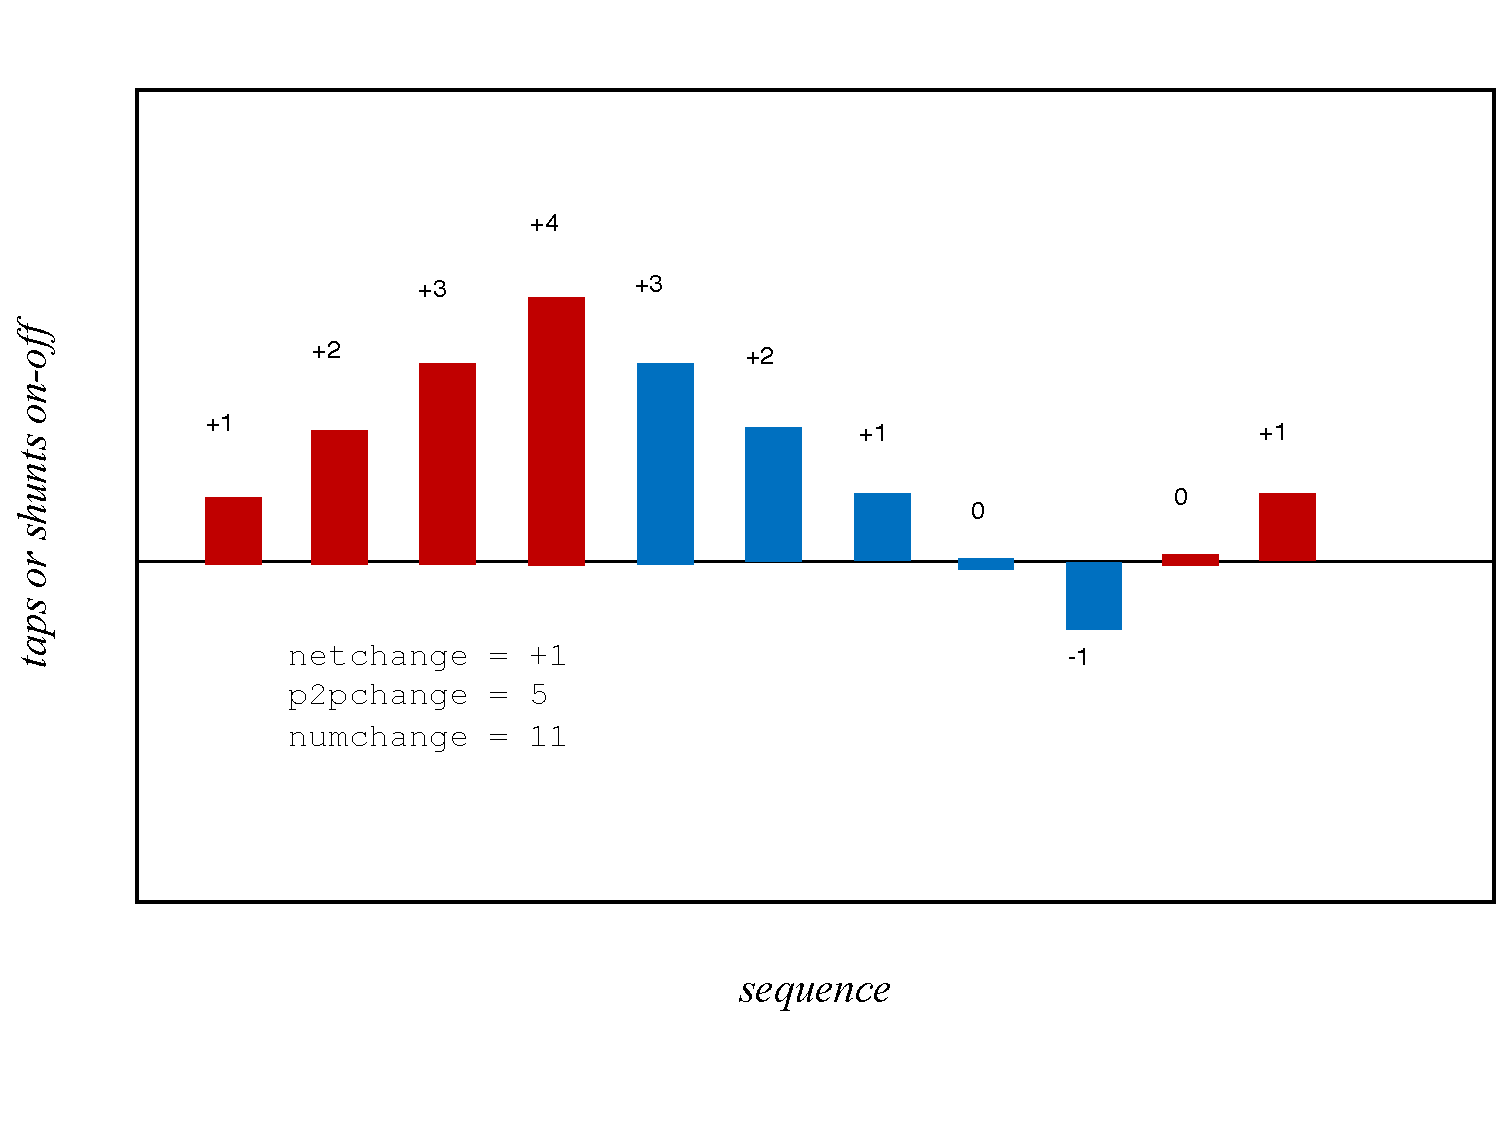
\includegraphics[width=\columnwidth]{figs/transient_characteristics_2}
  \caption{Our selection of reduced parameters for characterizing a
    sequence of binary (up/down, on/off) events.}
  \label{fig:tcharacteristics2}
\end{figure}



\subsubsection{Designing the metrics}
\label{sssec:metrics}
With the above selected variables and the defined reduced parameters,
there's 25 different categories (5 variable types x 5 reduced
parameters) for curves. In each category, there's usually more than
one data point. For instance, if there are 30 SVC controls in the case
file, there will be 30 pilot bus voltages. We have to choose a metric
in order to reduce the distances to a single number. Our preferred
choice is using \code{max(abs(diffs))}, which is the max-norm (also
called the L-infinity norm).  A different choice could be
\code{mean(abs(diffs))}, which is like the L1 norm divided by the
number of variables, but this choice smooths out important differences
when they are localized (which is normally the case when running a
very large network.)

For automata events, there is 8 categories:
\begin{itemize}
\item shunt\_netchanges: L1-norm of netchange diffs, normalized by the number of shunts
\item shunt\_numchanges: L1-norm of numchange diffs, normalized by the number of shunts
\item tap\_netchanges: L1-norm of netchange diffs, normalized by the number of transformers
\item tap\_p2pchanges: L1-norm of p2pchange diffs, normalized by the number of transformers
\item tap\_numchanges:  L1-norm of numchange diffs, normalized by the number of transformers
\item ldtap\_netchanges:  L1-norm of netchange diffs, normalized by the number of load-transformers
\item ldtap\_p2pchanges: L1-norm of p2pchange diffs, normalized by the number of load-transformers
\item ldtap\_numchanges: L1-norm of numchange diffs, normalized by the number of load-transformers
\end{itemize}  

We can think of this ``normalized L1 norm'' as being the same as
\code{mean(abs(diffs))}, only that the number of variables we are
using is \emph{all} devices that could potentially produce events, not
just the ones that have actually produced events. This way the metric
can tell apart cases where the number of devices involved in changes
is very different.


\subsubsection{Effective visualizations}
\textcolor{red}{TODO:} Briefly mention the role of effective viz for
experimenting with different metrics. Crucially: distinguish between
outliers vs.\ systematic diffs.  Then, point to the examples shown in
the next section.  There, show fig of main graph, the bubble scatter
plot of Astre vs.\ DynaWaltz values of the reduced parameters (which
is linked dynamically to the curve graph of specific points when
clicking on a bubble point).  Also, the graphs of the time evolution
of the difference in the number of automata changes (for each
category).



\subsubsection{Compound scoring and validation thresholds}

Compounding the 25 + 8 different categories into an aggregate metric
needs to be done carefully, in order to deal with the ``apples vs. oranges''
problem. Using relative error for each category sidesteps this problem (but
brings others).  On the other hand, from the point of view of validation, it is
more natural to define a set of thresholds, one in each of those 25+8
categories, using absolute error (one may later decide whether to assign a
global pass/not-pass based on some supra-metric on each individual pass/not-pass
value).

Tentatively, we have found the following thresholds (for absolute
errors) to be reasonable.
\begin{itemize}
\item V: 0.01 in pu
\item K: 0.1 (dimensionless)
\item P: 5 MW
\item Q: 5 MW
\end{itemize}

These thresholds are considered for characteristics dSS and dPP
(columns \code{dSS\_pass} and \code{dPP\_pass} in the notebook and
reports).  However, keep in mind that if they are used for
establishing a strict a pass/not-pass criteria, then it is found that
approximately up to 20\% of contingency cases fail the test. One may
want to play around with the thresholds in order to see how this
percentage varies.



\subsection{DynaFlow metrics}

Compared to dynamic simulations, the problem of establishing metrics
for comparing power flow solutions is, at first sight, comparatively
easier. If one only focuses on the electrical steady state, the
comparison can take place on the main variables: voltage magnitude at
buses, real \& active power flows through branches, and real \& active
power injections at buses (aggregate values, to sidestep modeling
differences due to merged loads, for instance). We then use the
L1-norm on the differences, either in absolute value or as a relative
error--looking at both is often necessary to uncover the most relevant
differences. As before, we do this separately for each magnitude type
and then define some compound scoring in order to mix all types into a
single figure, so that a single ranking of the ``top X worst
cases'' may be obtained.

More interesting for DynaFlow, though, is to detect discrete events
and activations of automatic controls in the simulation (relays, taps,
shunts, etc.).  When these take place, the differences between Hades
and DynaFlow solutions may be too large and uninformative, since the
case conditions may have diverged too much.  Looking at the timeline
of events is then needed in order to make sense of the results.
Metrics on the differences between power flow solutions are not helpful
in this case---it is simply better to detect the presence and number
of such events.  In particular, it is useful to try detecting ``root
cause'' events, that is, any significant event that in turn produces
several other events in a cascade.  We are currently researching on
this issue, since such cause--effect relationships are hard to ascribe
from the raw timeline of events without a proper electrical
analysis. We therefore devised a heuristic based on the distance
between events in time and space (i.e., distance measured by minimal
impedance paths across the grid), with which one can group these
events.  Even with ``false positives'', this kind of detection is
proving useful when investigating cases with large differences.

On the other hand, if one is comparing DynaFlow vs.\ DynaFlow results
then all time-domain information (events and curves) is kept, because
then all metrics and comparisons discussed above for the case of
DynaWaltz can be applied here as well.





%%%%%%%%%%%%%%%%%%%%%%%%%%%%%%%%%%%%%%%%%%%%%%%%%%%%%%%%%%%%%%%%%%%%%%%%%%%%%%%%
\section{Use cases and some sample results}

Originally the tool was designed for validating DynaWaltz on large
networks by means of comparison with an established simulator (Astre)
over a large set of contingency cases. Other use-cases were later
added: comparing DynaWaltz vs.\ DynaWaltz cases, either for validating
new versions or for experimenting with new models; and the screening
of contingencies, either for reducing the test set in automated
validation studies, or as an aim in itself.  All of these use-cases
were extended and carried over to the power flow solver, DynaFlow.

The pipeline results are shown in both graphical and tabular form in a
Jupyter notebook designed for interaction.  Upon running this
notebook, the eyes are drawn to the plot in
Fig.~\ref{fig:bubbleplot1}.  This is one of the most useful graphs
in the notebook; it is an X-Y scatter plot of the reduced magnitude of
choice (dSS, dPP, TT, period, damping), for the signal class of
choice: contingency bus voltages, pilot bus voltages, generator P/Q,
or SVC control gain K-levels. The point color encodes the signal's
transient length, while the size encodes its peak-to-peak amplitude.
When the simulator results are the same, all dots accumulate on the
diagonal. Any differences are clearly visible as deviations from the
diagonal, and the point positions together with their color and size
quickly inform the user about the severity of each contingency case.

\begin{figure}
  \centering
  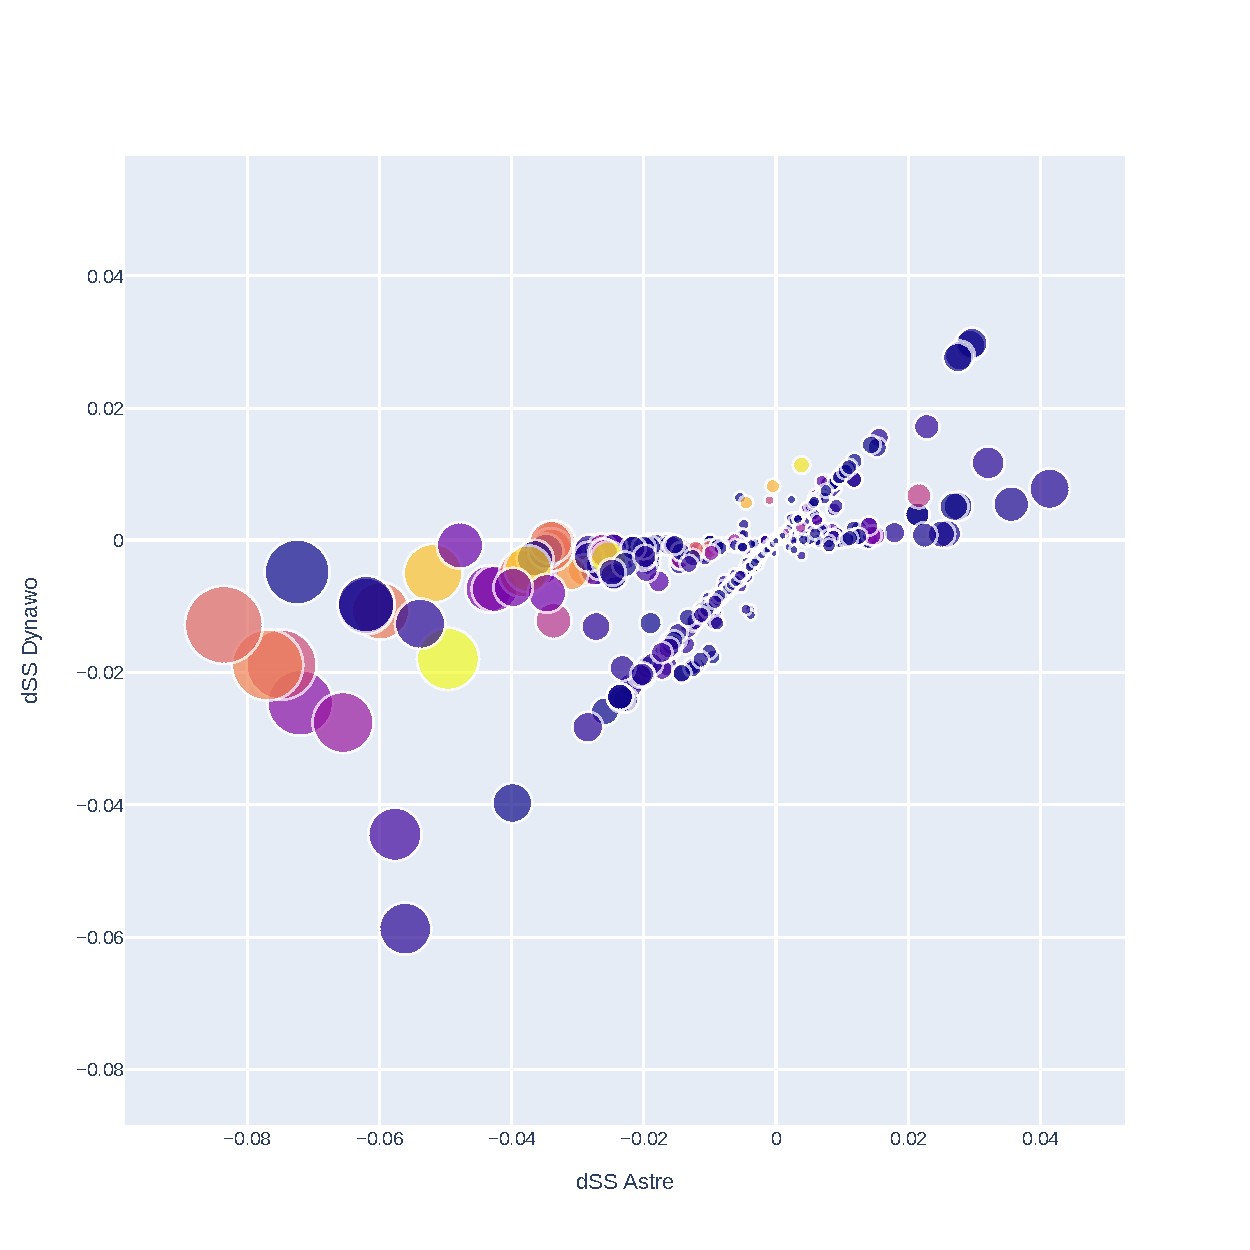
\includegraphics[width=\columnwidth]{figs/Ubus_dSS_GENS_20210211-0930_moreT600}
  \caption{Scatter plot of dSS (change in steady state) of the bus
    voltage at the contingency point, for single-generator contingency
    cases (exhaustive N-1 contingency run: 4,577 cases). The point
    color encodes the signal's transient length; the size encodes its
    peak-to-peak amplitude.}
  \label{fig:bubbleplot1}
\end{figure}

The power of this plot lies in that it synthesizes the globality of
results.  It is useful to detect outliers but, more importantly, it is
also very effective at revealing \emph{systematic} differences, that
is, patterns in the deviations, which typically signal some sort of
modeling differences. Figure~\ref{fig:bubbleplot1} shows an example of
this: a significant number of buses accumulate on a small slope line
away from the diagonal, possibly indicating that the generators near
the contingency have some sort of modeling differences in their
voltage control. Hypotheses such as this can quickly be put to the
test by exploring the plot. Hovering over each point reveals the
device's information (ID, voltage level, etc.), and clicking on it
automatically selects the particular contingency case and device
signal to plot on the rest of the graphs. This allows one to quickly
to drill down to specific curve graphs and analyze behaviors.

Visual inspection of the curve graphs is always useful as a
double-check on a number of things. For instance, during development
we once found many unexpected outliers, but a quick look at their
curves quickly showed that the steady-state had not yet been achieved
at the end of the run. If this happens, metrics for the differences
are bound to be very large and completely meaningless.  This prompted
us to improve our mechanisms for detecting and flagging unstable
cases, so that they can be removed from the comparison.

The tabular information is also there in the notebook, in case one
wants to have access to the actual values and metrics. It is presented
in data grid widgets that allow for sorting and filtering.  These
values are also exported to CSV files, for further analysis in other
tools such as Excel.  Data tables are particularly useful for ranking
contingencies by means of the compound scoring metrics discussed in
the previous section.

As a brief example of how to analyze results with the notebook, let us
take a look at the examples in Figs.~\ref{fig:bubbleplot2} and
~\ref{fig:curveplot}. In this case the scatter plot represents the
reactive power injection (Q) of all generators participating in the
coordinated secondary voltage control (SVC) systems. There seems to be
no significant patterns of systematic differences, such as lines or
clusters off the diagonal, but there are several outliers sprinkled
here and there.  As we become interested in any of these, we click on
it and the graphs in Fig.~\ref{fig:curveplot} update to show the
specific information for the chosen generator, under the specific
contingency case. The time-domain signal shows indeed a net difference
of about 60 Mvar in output, once the new steady state is reached. The
graph stacked on top shows the metrics for the global differences in
discrete events vs.~simulation time (see subsection~\ref{sssec:metrics}
above).  In this case we observe that shunt and tap events do not
differ much after the contingency, meaning that the differences in Q
developing after t$\sim$1,100s must be due to purely local effects. This
prompts us to investigate the model of this generator further, and to
try finding whether there are commonalities shared by other outliers of
this kind, etc.

\begin{figure}
  \centering
  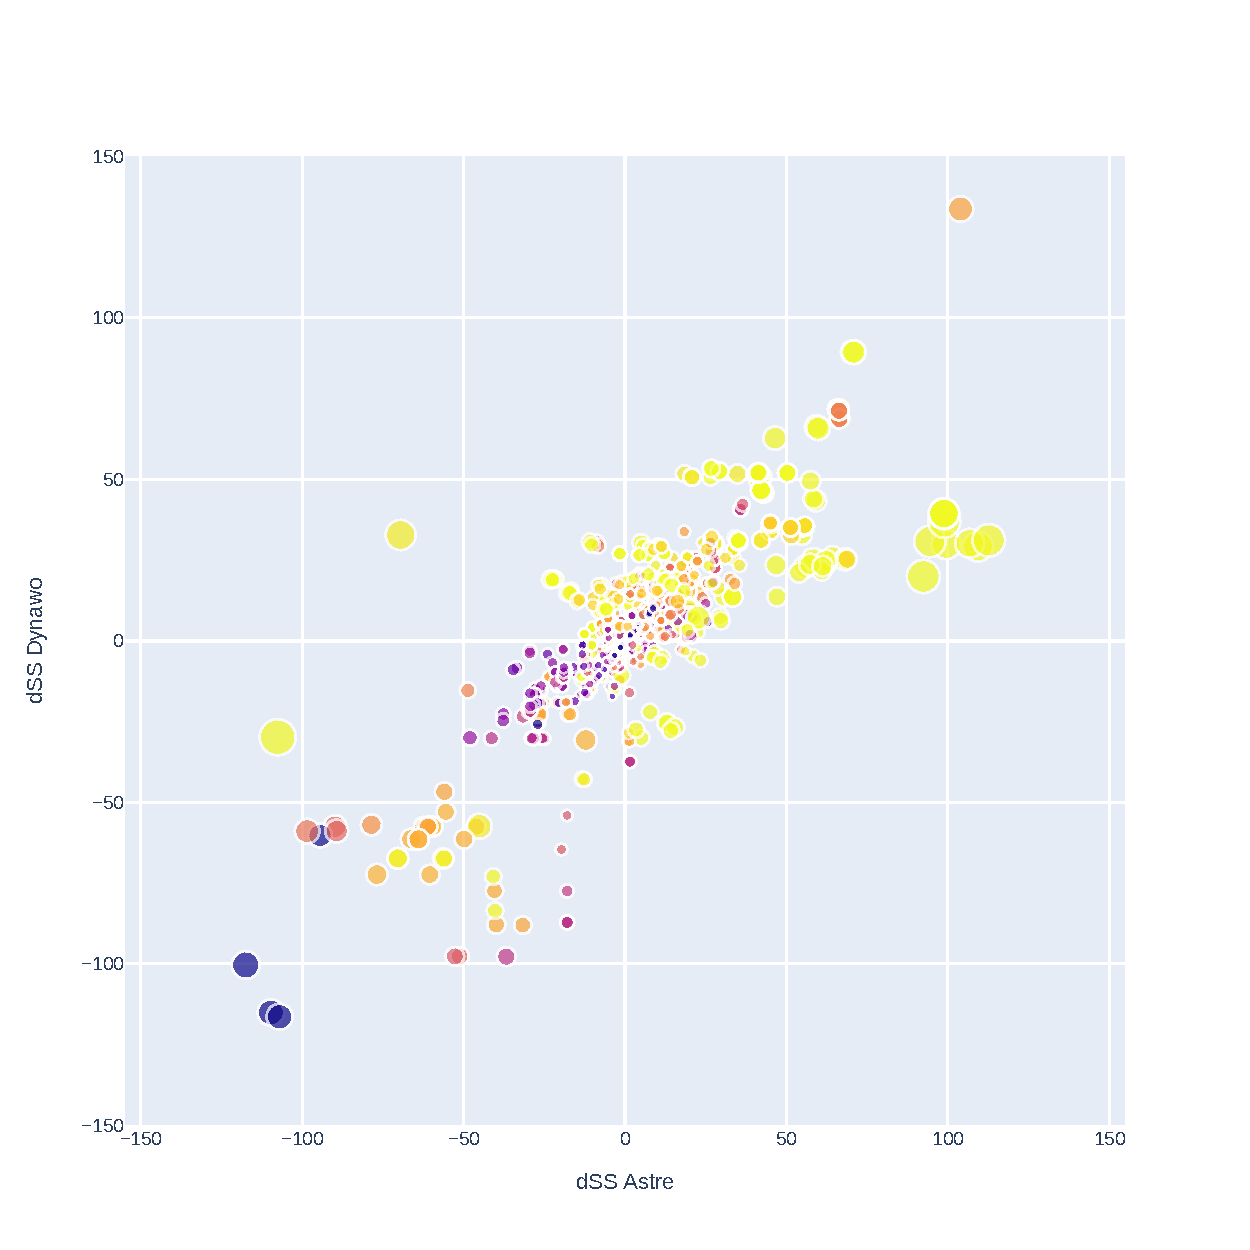
\includegraphics[width=\columnwidth]{figs/Qgen_dSS_GENS_20210211-0930_moreT600}
  \caption{Same as Fig.~\ref{fig:bubbleplot1}, but for dSS in the Q
    injected by the generators participating in the coordinated
    secondary voltage control systems.}
  \label{fig:bubbleplot2}
\end{figure}

\begin{figure}
  \centering
  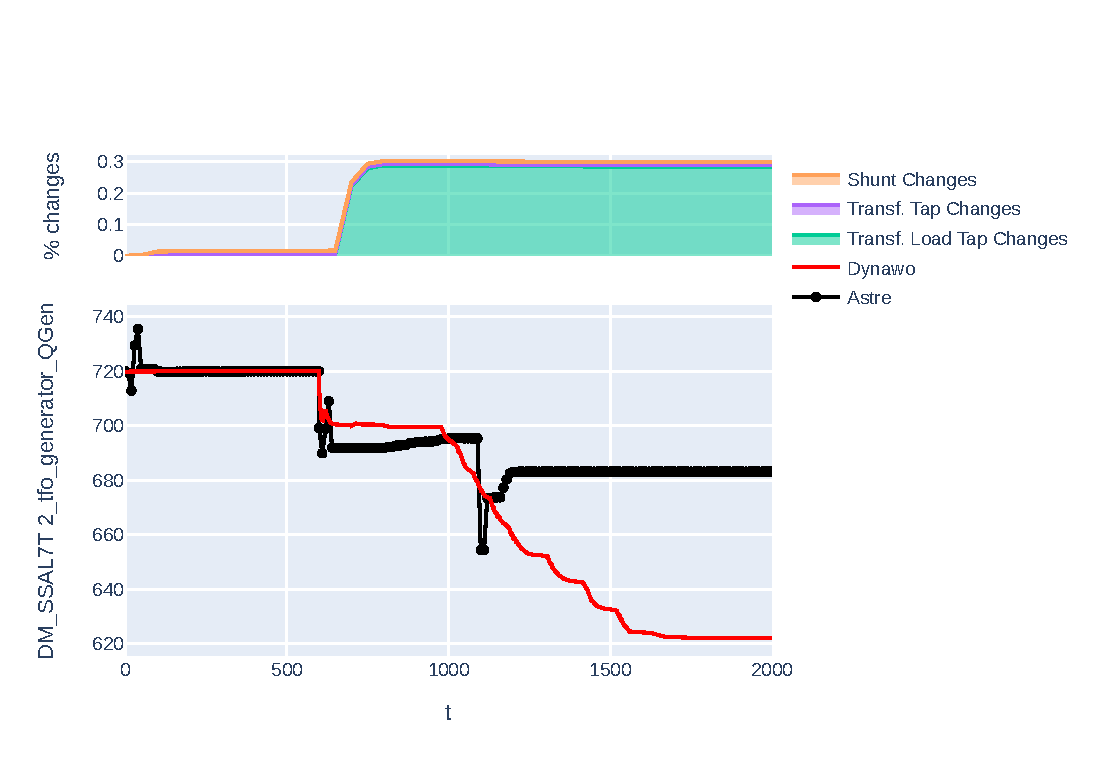
\includegraphics[width=\columnwidth]{figs/Qgen_curve_GENS_20210211-0930_moreT600}
  \caption{Bottom plot: injected reactive power (Q) of a generator
    participating in SVC (contingency takes place at t=600s). Top
    plot: global metrics for the differences in events vs.\ time.}
  \label{fig:curveplot}
\end{figure}




%%%%%%%%%%%%%%%%%%%%%%%%%%%%%%%%%%%%%%%%%%%%%%%%%%%%%%%%%%%%%%%%%%%%%%%%%%%%%%%%
\section{Technical notes}

This tool is intentionally architected as a collection of loosely
coupled scripts, mixing Python and Bash shell scripting. The rationale
behind this choice is that we wanted to retain the flexibility to
perform large changes, as this was to be a tool for research as much
as a tool for automatic validation tests. Nevertheless, the tool is
packaged as a proper Python package, for easy management of all the
dependencies. Installation is simply a matter of pip-installing the
package, taking up around 900MB of disk space on a clean virtual env.
Note that we did not use an \emph{application} installer, since this
is not a closed, monolithic application; instead, we want to promote
further development and easy customization though modularity.

As for the graphical part, we decided to use Jupyter
notebooks~\cite{jupyter_nb} instead of dashboard-style application
frameworks, for similar reasons. We wanted to retain the ability to
quickly code up new graphs or new functionality, and working with
notebooks has very quick turnaround times while also allowing some
interactive, dashboard-style widgets.  Still, we were careful to
separate as much code as possible into Python modules, instead of
polluting the notebook. This is important because one of the big
disadvantages of notebooks, from the point of view of software
engineering practices, is that they make it very cumbersome (even
impossible) to work with version control, code linters, profilers, and
unit testing.

In terms of proper coding practices, we use flake8~\cite{flake8} and
shellcheck~\cite{shellcheck} as our main linters, occasionally using
  Pylint~\cite{pylint} and PyCharm's~\cite{pycharm} checks as
  well. For Python code formatting, we used Black~\cite{black}.

Notable dependencies in our code, due to their usefulness, are
Pandas~\cite{pandas}, NumPy~\cite{numpy}, and
NetworkX~\cite{networkX}.  Launching many simulator instances in
parallel is enabled thanks to GNU parallel~\cite{GNUparallel}, a very
robust and flexible utility. For graphics, we opted for Plotly due to
its maturity, wide selection of chart types, and their interactivity
through IPython widgets.  The only downside encountered is that Plotly
charts start showing bad performance when the number of points in the
chart go over approximately 5,000.  This is the case in
Figs.~\ref{fig:bubbleplot1} and \ref{fig:bubbleplot2}: since we
routinely deal with contingency runs exceeding 12,000 cases, each
having more than 30 variables in each class, we had to devise ways to
intelligently reduce those $\sim$360,000 points to something more
manageable: a small algorithm to dynamically remove non-interesting
points, i.e.~those close to the diagonal and to the origin.

The tool is expected to be released soon as Open Source, under the
umbrella of all the other \Dynawo projects~\cite{DwoGitRepos}.




%%%%%%%%%%%%%%%%%%%%%%%%%%%%%%%%%%%%%%%%%%%%%%%%%%%%%%%%%%%%%%%%%%%%%%%%%%%%%%%%
\section{Conclusion}

We have presented a tool for the testing and validation of dynamic
simulators DynaWaltz and DynaFlow on large, real-world transmission
networks.  Our approach is based on the extensive simulation of
contingency cases, comparing the results to another
already-established simulator acting as a reference. The tool may also
be used for testing new versions of the software (i.e., as a
complement to Unit Testing); or for exploring the effects of different
modeling choices, model parameters, solver parameters, etc., on the
behavior of the whole network.  Besides supporting manual analysis of
results, the tool can be used for deploying automated testing
procedures to help evolving the software, the models, and their
parameterization.

To meet the challenges involved in taking quantitative measurements of
the differences between simulations, in ways that make sense from the
electrical point of view, we researched on how to select the most
relevant output values, along with the corresponding metrics to assess
the distance between two results. In the case of DynaWaltz, this
involved the distillation of data into a reduced set of parameters
that characterize the most relevant features of the time-domain
signals.  Another challenge was dealing with such large amounts of
data efficiently, and designing effective visualizations for the
results. For this, we leveraged several modern libraries and rapid
development tools from the Python ecosystem.




%%%%%%%%%%%%%%%%%%%%%%%%%%%%%%%%%%%%%%%%%%%%%%%%%%%%%%%%%%%%%%%%%%%%%%%%%%%%%%%%
%% \section*{Acknowledgment}
%% Any thanks/ack to funding bodies? (Linux Foundation Energy?)




%%%%%%%%%%%%%%%%%%%%%%%%%%%%%%%%%%%%%%%%%%%%%%%%%%%%%%%%%%%%%%%%%%%%%%%%%%%%%%%%
\bibliographystyle{IEEEtran}
\bibliography{IEEEabrv,dynawo_validation}




\end{document}




%% Place figures and tables at the top and bottom of columns. Avoid placing them in
%% the middle of columns. Large figures and tables may span across both
%% columns. Figure captions should be below the figures; table heads should appear
%% above the tables. Insert figures and tables after they are cited in the
%% text. Use the abbreviation ``Fig.~\ref{fig}'', even at the beginning of a
%% sentence.
%%
%% \begin{table}[htbp]
%%   \caption{Table Type Styles}
%%   \begin{center}
%%     \begin{tabular}{|c|c|c|c|}
%%       \hline
%%       \textbf{Table}&\multicolumn{3}{|c|}{\textbf{Table Column Head}} \\
%%       \cline{2-4} 
%%       \textbf{Head} & \textbf{\textit{Table column subhead}}&
%%       \textbf{\textit{Subhead}}& \textbf{\textit{Subhead}} \\
%%       \hline
%%       copy& More table copy$^{\mathrm{a}}$& &  \\
%%       \hline
%%       \multicolumn{4}{l}{$^{\mathrm{a}}$Sample of a Table footnote.}
%%     \end{tabular}
%%     \label{tab1}
%%   \end{center}
%% \end{table}

%% \begin{figure}[htbp]
%%   \centerline{\includegraphics{fig1.png}}
%%   \caption{Example of a figure caption.}
%%   \label{fig}
%% \end{figure}

